
\section{Spatial Election}

\begin{enumerate}
\def\labelenumi{\arabic{enumi}.}
\item
  Project
\item
  \href{https://github.com/a-d/spatial.election/wiki/Description-and-Setup}{Description}
\item
  Implementation
\item
  \href{https://github.com/a-d/spatial.election/wiki/Strategy}{Strategy}
\item
  Implementation Details

  \begin{enumerate}
  \def\labelenumii{\arabic{enumii}.}
  \itemsep1pt\parskip0pt\parsep0pt
  \item
    \href{https://github.com/a-d/spatial.election/wiki/Datenmodell}{Data
    Model}
  \item
    \href{https://github.com/a-d/spatial.election/wiki/Database-Layer}{Database
    Layer}
  \item
    \href{https://github.com/a-d/spatial.election/wiki/Constituencies-and-Counties}{Constituencies
    and Counties}
  \item
    \href{https://github.com/a-d/spatial.election/wiki/Frontend}{Frontend}
  \end{enumerate}
\item
  Installation
\item
  \href{https://github.com/a-d/spatial.election/wiki/Setup-Eclipse}{Setup
  Eclipse}
\item
  \href{https://github.com/a-d/spatial.election/wiki/Setup-PostgreSQL}{Setup
  PostgreSQL}
\item
  \href{https://github.com/a-d/spatial.election/wiki/Running}{Running}
\item
  Demonstration
\item
  \href{http://178.254.23.23:9191/}{Live spatial.election Server}
\item
  \href{postgresql://178.254.23.23:5432}{Live spatial.election Database}
\item
  \href{http://userpage.fu-berlin.de/~al3x/spatial.election.war}{Mirror
  spatial.election WAR}
\item
  \href{http://userpage.fu-berlin.de/~al3x/spatial.election.jar}{Mirror
  spatial.election JAR}
\end{enumerate}

\begin{center}\rule{3in}{0.4pt}\end{center}

\begin{figure}[htbp]
\centering
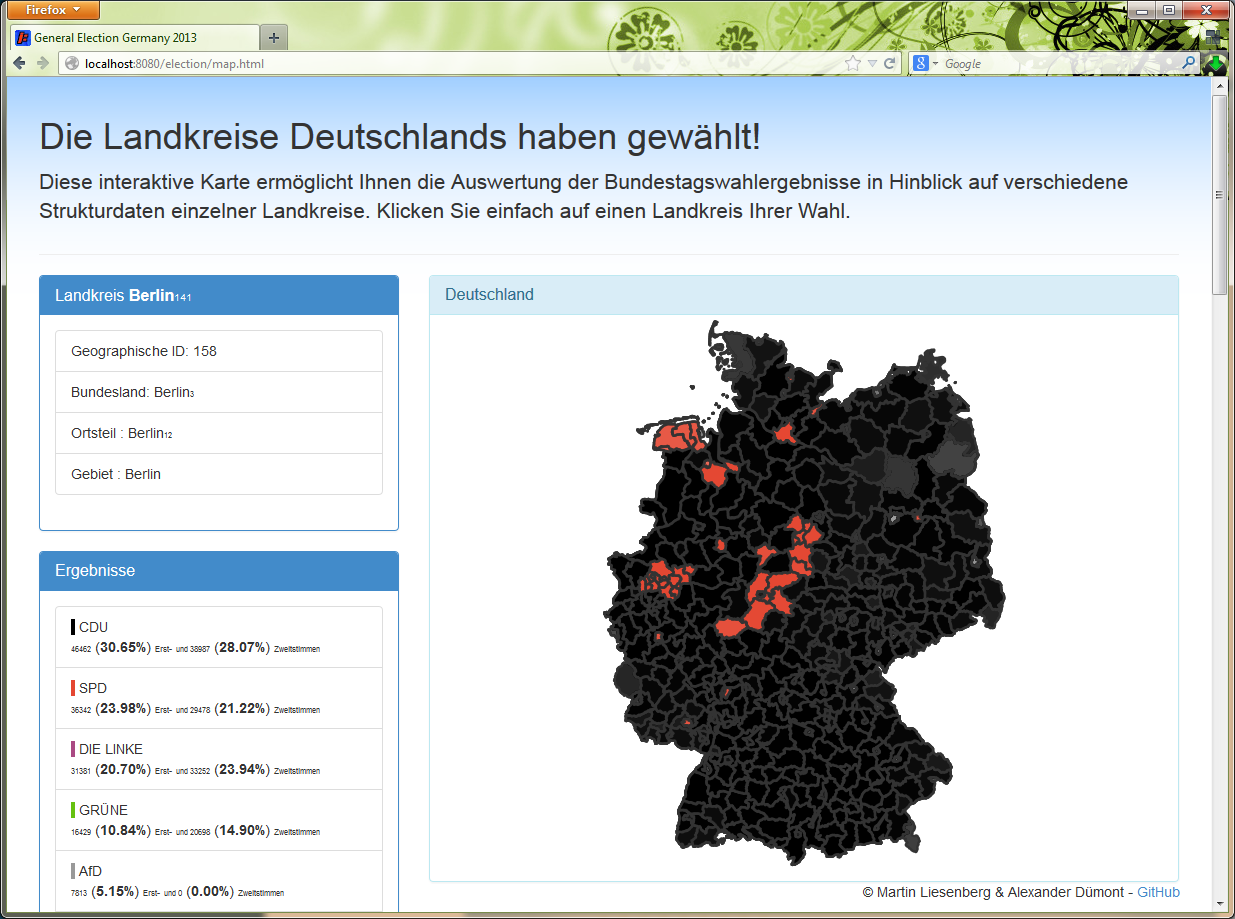
\includegraphics[width=1.2\textwidth]{../img/JKGj20F.png}
\caption{image}
\end{figure}